\documentclass{standalone}
\usepackage{tikz}
\usepackage{ctex,siunitx}
\usepackage{tkz-euclide}
\usepackage{amsmath}
\usetikzlibrary{patterns, calc}
\usetikzlibrary {decorations.pathmorphing, decorations.pathreplacing, decorations.shapes,}
\begin{document}
\small
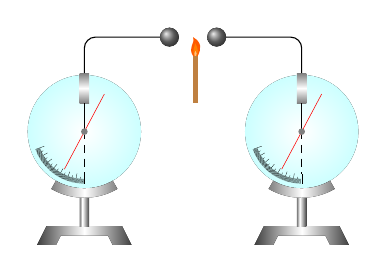
\begin{tikzpicture}[>=latex,scale=1.2]
  % \useasboundingbox(-1,-2)rectangle(8,6);
  \fill[inner color=white, outer color=cyan!20](0,0)circle(0.6);
  \fill[left color=darkgray,right color=darkgray, middle color=white](-0.5,-1.2)--++(0.2,0)--++(0.05,0.1)--++(0.5,0)--++(0.05,-0.1)--++(0.2,0)--++(-0.1,0.2)--++(-0.8,0)--cycle;
  \fill[left color=gray,right color=white](-0.05,-0.6)rectangle(-0.02,-1.0);
  \fill[left color=white,right color=darkgray](-0.02,-0.6)rectangle(0.05,-1.0);
  \fill[left color=gray,right color=gray, middle color=white](300:0.6)arc(300:240:0.6)--(240:0.7)arc(240:300:0.7)--cycle;
  \fill[top color=gray,bottom color=gray,middle color=white](-0.05,0.3)rectangle(0.05,0.62);
  \draw[rounded corners](0,0.62)--(0,1.0)--(0.8,1.0);
  \draw(0,0.3)--(0,0);
  \draw[very thin,densely dashed](0,0.3)--(0,-0.45);
  \draw[very thin,red](62:0.45)--(242:0.45);
  \fill[gray](0,0)circle(1pt);
  \foreach \x in {200,210,...,260}
  {
    \draw[ultra thin](\x:0.55)--(\x:0.45);
    \foreach \y in {1,2,3,4,6,7,8,9}
    {\draw[ultra thin](\x+\y:0.55)--(\x+\y:0.5);}
    \draw[ultra thin](\x+5:0.55)--(\x+5:0.48);
  }
  \draw[ultra thin](270:0.55)--(270:0.45);
  \fill[ball color=gray](0.9,1.0)circle(0.1);
  \begin{scope}[xshift=2.3cm]
    \fill[inner color=white, outer color=cyan!20](0,0)circle(0.6);
    \fill[left color=darkgray,right color=darkgray, middle color=white](-0.5,-1.2)--++(0.2,0)--++(0.05,0.1)--++(0.5,0)--++(0.05,-0.1)--++(0.2,0)--++(-0.1,0.2)--++(-0.8,0)--cycle;
    \fill[left color=gray,right color=white](-0.05,-0.6)rectangle(-0.02,-1.0);
    \fill[left color=white,right color=darkgray](-0.02,-0.6)rectangle(0.05,-1.0);
    \fill[left color=gray,right color=gray, middle color=white](300:0.6)arc(300:240:0.6)--(240:0.7)arc(240:300:0.7)--cycle;
    \fill[top color=gray,bottom color=gray,middle color=white](-0.05,0.3)rectangle(0.05,0.62);
    \draw[rounded corners](0,0.62)--(0,1.0)--(-0.8,1.0);
    \draw(0,0.3)--(0,0);
    \draw[very thin,densely dashed](0,0.3)--(0,-0.45);
    \draw[very thin,red](62:0.45)--(242:0.45);
    \fill[gray](0,0)circle(1pt);
    \foreach \x in {200,210,...,260}
    {
      \draw[ultra thin](\x:0.55)--(\x:0.45);
      \foreach \y in {1,2,3,4,6,7,8,9}
      {\draw[ultra thin](\x+\y:0.55)--(\x+\y:0.5);}
      \draw[ultra thin](\x+5:0.55)--(\x+5:0.48);
    }
    \draw[ultra thin](270:0.55)--(270:0.45);
    \fill[ball color=gray](-0.9,1.0)circle(0.1);
  \end{scope}
  \fill[red!30!orange](1.200,0.800)..controls(1.240,0.883)and(1.243,0.943)..  (1.150,1.000)..controls(1.175,0.923)and(1.091,0.901)..(1.150,0.800)--cycle;
  \fill[orange](1.163,0.800)..controls(1.141,0.869)and(1.168,0.888)..
  (1.172,0.937)..controls(1.209,0.871)and(1.207,0.841)..(1.188,0.800)--cycle;
  \fill[orange!50](1.181,0.800)..controls(1.191,0.821)and(1.192,0.836)..
  (1.176,0.854)..controls(1.172,0.844)and(1.158,0.835)..(1.169,0.800)--cycle;
  \fill[brown](1.15,0.8)rectangle++(0.05,-0.5);
\end{tikzpicture}
\end{document}